\subsubsection{Digitiztaion of the Hadronic Veto System (Editors: Nhan Tran, Andrew Whitbeck)}
\label{sec:hcaldig}

After full {\tt GEANT4} simulation, we simulate the digitization of the particle-level interactions in our detector to 
understand how well we can reconstruct events in the hadronic calorimeter.  Given the particle-level energy 
deposition per layer, we can convert that into the an expected number of photo-electrons (PEs).   
{\tt GEANT4} simulations with 4 GeV incident muons are used to estimate the expected detector response to minimum ionizing particles (MIPs).  Fig.~\ref{fig:hcalMIP} shows the distribution of energy deposited in a given layer of scintillator; on
average, each MIP deposits 1.4 MeV of energy in a given layer.   For each MIP, we assume that 20 PEs are detected
on average.

The digitization parameters used in these studies are based on CMS test beam measurments~\cite{}, where 
the mean MIP response was 13.5 PEs for a comparable HCal geometry.  This MIP response has been scaled up to
account for the differences in scintillator thinkness, assuming that the light collection efficiency will remain constant.

The sum of SiPM and electronics noise is expected to be 2 PEs.  Although noise is not explicitly simulated, only layers
that have a minimum of 8 PEs are considered in further studies.   Thus, noise affects are expected to be negligible.  



\begin{figure}[hbtp]
\begin{center}
    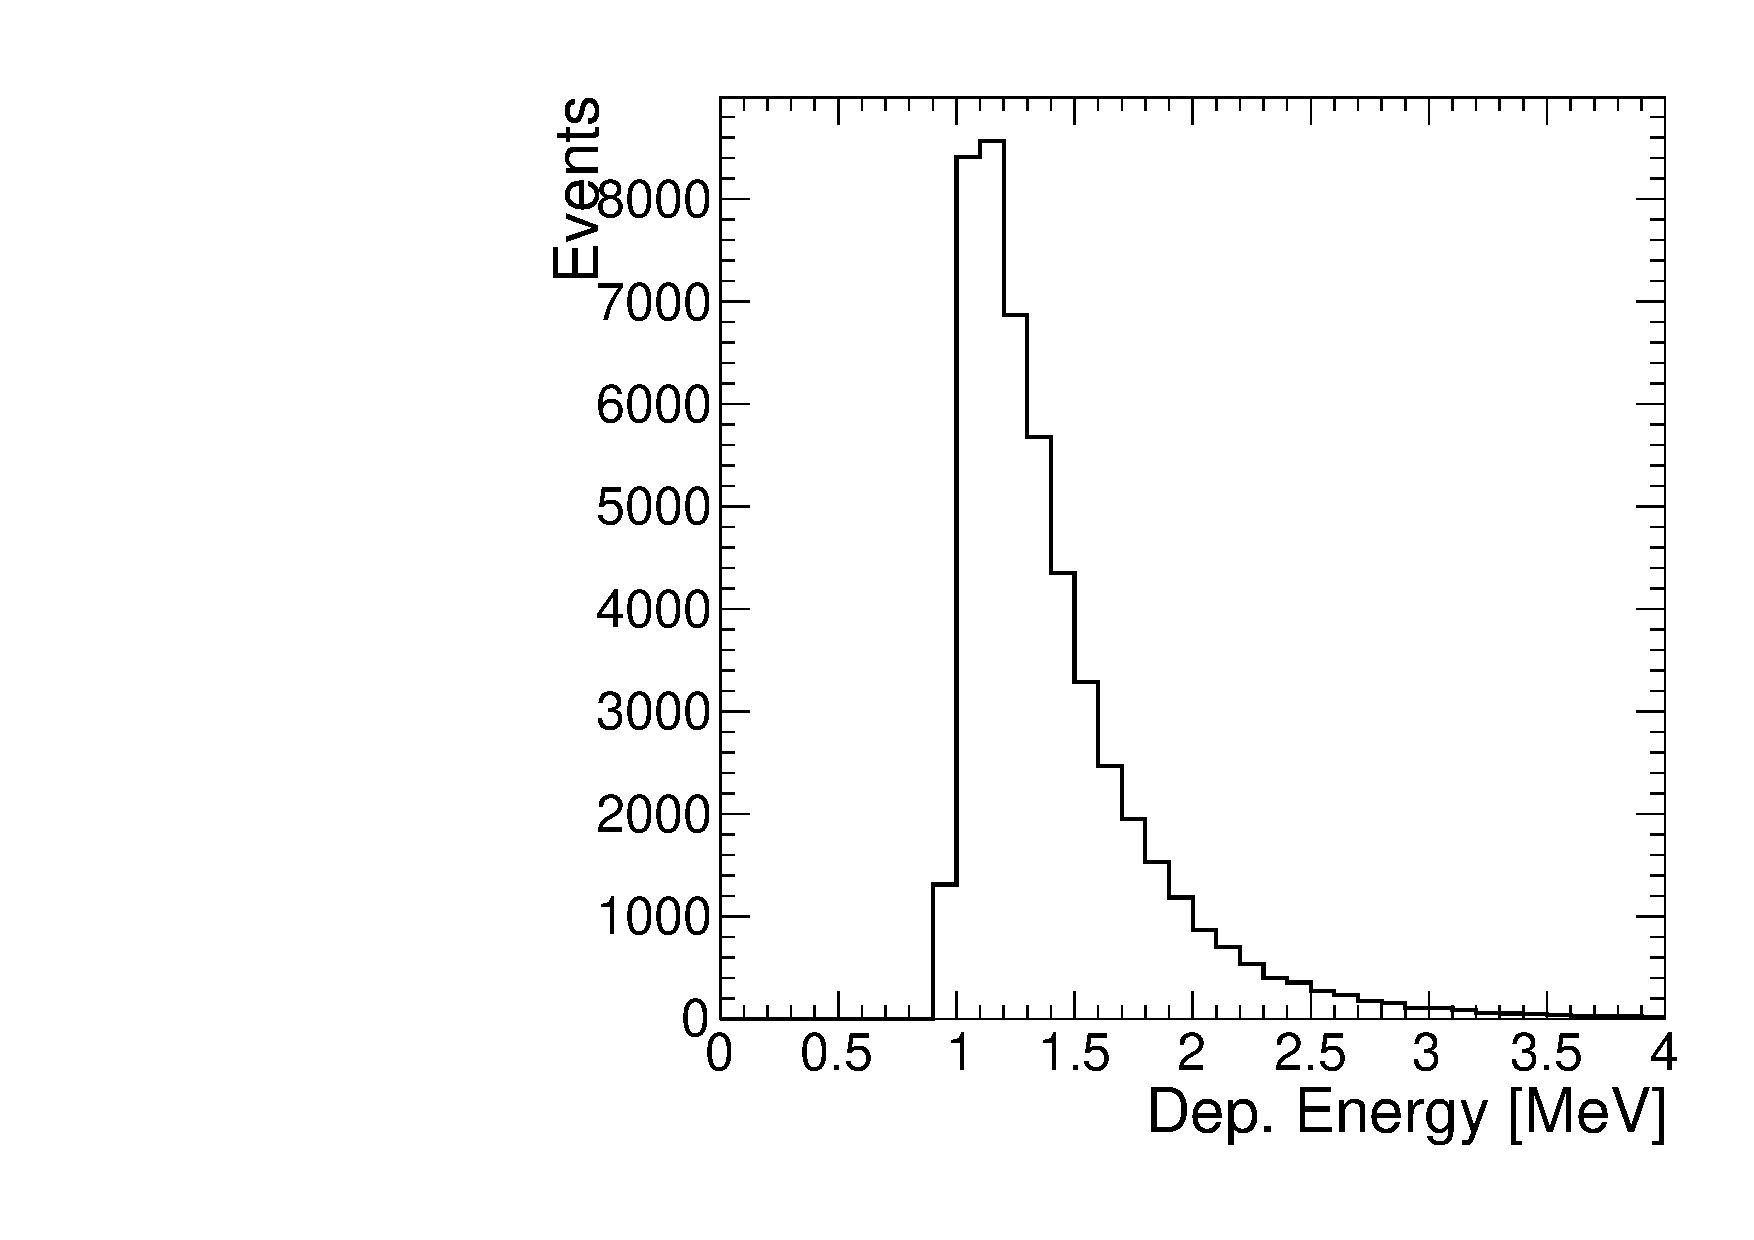
\includegraphics[width=0.5\textwidth]{images/hcal/MIPresponse0degreesOnly.pdf}
    \caption{Distribution of energies deposited in scintillator from muon to characterize MIP behavior in plastic scintillator}
 \label{fig:hcalMIP}
 \end{center}
\end{figure}
